\documentclass{article}
%% Useful packages
\usepackage[utf8]{inputenc}
\usepackage[a4paper,left=2cm,right=2cm,top=2cm,bottom=2cm]{geometry}
\usepackage{crop,graphicx,array,color,amssymb,fancyhdr,lineno}
\usepackage{flushend,stfloats,amsthm,chngpage,times,lipsum,lastpage} 
\usepackage{calc,listings,color,wrapfig,tabularx,longtable,enumitem}
\usepackage[style=numeric-comp,backend=biber]{biblatex}
\usepackage{lineno}
\usepackage{parskip}
\usepackage[fleqn]{amsmath}
\usepackage{caption}
\usepackage{subcaption}
\usepackage{float}
\usepackage{titlesec}
\usepackage{colortbl}
\usepackage{tikz}
%%%%%%%%%%%%   Header and Footer  %%%%%%%%%%%%%
\pagestyle{fancy}
\fancypagestyle{plain}{%
	\renewcommand{\headrulewidth}{0pt}%
	\fancyhf{}%
}

\begin{document}
	\begin{titlepage}
	
	\newcommand{\HRule}{\rule{\linewidth}{0.5mm}} % Defines a new command for the horizontal lines, change thickness here
	\newcommand{\MyPath}{C:/Magistrale} %TODO Modificare questo path con la cartella di destinazione delle immagini
	
	%----------------------------------------------------------------------------------------
	%	LOGO SECTION
	%----------------------------------------------------------------------------------------
	\center

    \begin{figure}[h]
    \centering
    
\includegraphics[width=0.5\textwidth]{Immagini/logo_verticale_COLORE.png}
    \label{fig:logo_verticale_COLORE.png}
\end{figure}
	 % Include a department/university logo - this will require the graphicx package
	
	%----------------------------------------------------------------------------------------
	
	\center % Center everything on the page
	
	%----------------------------------------------------------------------------------------
	%	HEADING SECTIONS
	%----------------------------------------------------------------------------------------
	\vspace{1cm}
	\textsc{\LARGE DIBRIS}\\[0.3cm]
	\textsc{\small Department of Informatics,}\\
	\textsc{\small Bioengineering, Robotics and System Engineering}\\[1cm] % Minor heading such as course title
	\textsc{\LARGE{Mechanical Design Methods 2025/2026}}\\[1cm] % Major heading such as course name
	
	%----------------------------------------------------------------------------------------
	%	TITLE SECTION
	%----------------------------------------------------------------------------------------
	\makeatletter
	\HRule \\[0.4cm]
	{ \huge \bfseries Mechanical Design Methods - Report group 9}\\[0.2cm] 
	%{\Large \bfseries }\\
	% Title of your document
	\HRule \\[1.5cm]
	
	%----------------------------------------------------------------------------------------
	%	AUTHOR SECTION
	%----------------------------------------------------------------------------------------
	
	\begin{minipage}{0.4\textwidth}
		\begin{flushleft} \large
			\emph{Authors:}\\[0.2cm]
			Antonio Mazzotta - S8973098\\
			Francesco Sisani - S8571674\\
			Matteo Spluga - S9185902
			%[1.2em]
			%\emph{Student ID:}\\
			%[0.2cm]
			%s8973098\\
			%[1.2em]
		\end{flushleft}
	\end{minipage}
	~
	\begin{minipage}{0.4\textwidth}
		\begin{flushright} \large
			\emph{Professors:} \\[0.2cm]
			Matteo Zoppi\\ % Supervisor's Name
			Gabriele Reverberi\\[1.2em]
			
		\end{flushright}
	\end{minipage}\\[2cm]
	\makeatother
	
	% If you don't want a supervisor, uncomment the two lines below and remove the section above
	%\Large \emph{Author:}\\
	%John \textsc{Smith}\\[3cm] % Your name
	
	%----------------------------------------------------------------------------------------
	%	DATE SECTION
	%----------------------------------------------------------------------------------------
	
	
	\vfill % Fill the rest of the page with whitespace
	
\end{titlepage}
	
	\sffamily
	
	\fancyhf{}
	\fancyhead[L]{A. Mazzotta - F. Sisani - M. Spluga}
	\fancyhead[R]{Mechanical Design Methods - Report Group 9}
	\fancyfoot[R]{ \bf\thepage\ \rm }%
	
	\newpage
	\tableofcontents


	\newpage
	\section{Introduction}
For this project, it is requested to design a mechanical system that can lift a Rzeppa half-shaft constant velocity end joint with a specially designed gripper starting from the base frame of a \texttt{Jodell} gripper. The half-shaft joint is positioned on a tray designed according to its dimensions, from which the gripper will lift the same object.

\subsection{Constant Velocity joint}
A constant-velocity joint (also called a CV joint or homokinetic joint) is a mechanical connection between two rotating shafts, that keeps them rotating at the same speed, while allowing the shafts to be at an angle to each other as they rotate. This joint operates without an appreciable increase in friction or backlash and compensates for the angle between the two shafts, within a certain range of angles.
A common use of CV joints is in front-wheel drive vehicles, where they are used to transfer the engine's power to the front wheels while still allowing the wheels to steer.
A Rzeppa joint consists of a spherical inner shell with 6 grooves in it and a similar enveloping outer shell. Each groove guides one ball. The input shaft fits in the center of a large, steel, star-shaped "gear" that nests inside a circular cage. The cage is spherical but with ends open, and it typically has six openings around the perimeter. 

\subsubsection{Half-shaft end joint}
For this application, we consider a Rzeppa half-shaft constant velocity end joint. Due to its asymmetric structure, its mass is not equally distributed and the center of mass is shifted toward the bulkier head of the joint. Consequently, during lifting, the component tends to tilt under gravity. 

The main design challenge was to determine the optimal grasp location for the modified \texttt{Jodell} gripper while stabilizing the asymmetric load to prevent rotation. Since the joint is made of high-strength metals, structural deformation under clamping force was not a concern. Instead, the design focused on grasping the cylindrical shaft while the part lies horizontally on a custom tray, managing the gravity-induced momentum. Later in this report, we detail how this stabilization was resolved and how the gripper was dimensioned to accommodate a range of automotive shaft diameters.

Its principal measurements are: $90\text{ mm}$ for the head diameter, $23\text{ mm}$ for the threaded section, and $100\text{ mm}$ as the span for stabilization and grasping contacts. Specifically, the grasping claws operate on the intermediate $28\text{ mm}$ diameter (non-threaded) section of the cylinder, whereas the buffer stabilization system acts on the $23\text{ mm}$ diameter threaded section. Images of the physical component and the corresponding 3D CAD model (imported into Creo 9.0.10.0 from SolidWorks) are shown below.

\begin{figure}[H]
    \centering
    \begin{minipage}{0.43\textwidth}
        \centering
        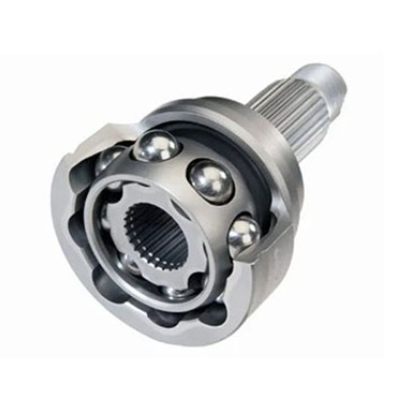
\includegraphics[width=\textwidth]{Immagini/Half-shaft/rzeppa half-shaft.png}
        \caption{Rzeppa's Half-shaft end joint}
    \end{minipage}
    \hfill
    \begin{minipage}{0.43\textwidth}
        \centering
        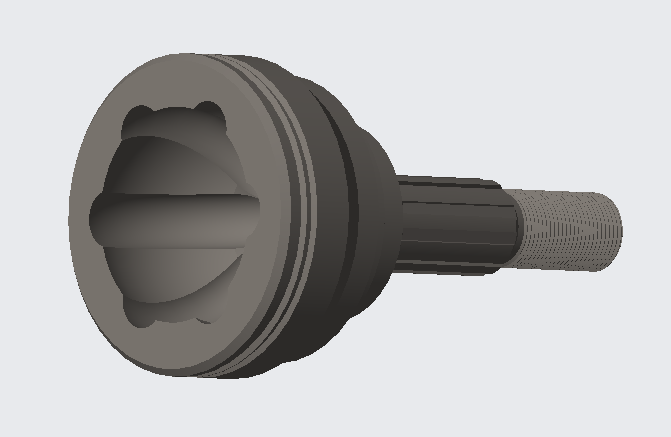
\includegraphics[width=\textwidth]{Immagini/Half-shaft/Half-shaft.png}
        \caption{Half-shaft end joint}
    \end{minipage}
\end{figure}

\begin{figure}[H]
    \centering
    \begin{minipage}{0.35\textwidth}
        \centering
        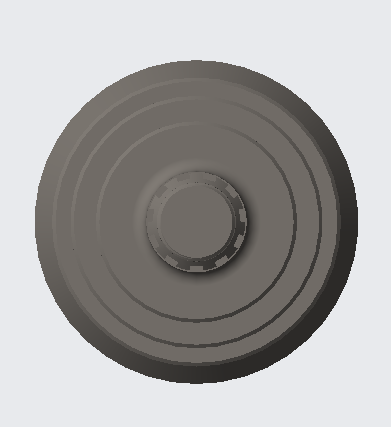
\includegraphics[width=\textwidth]{Immagini/Half-shaft/Half-shaft back .png}
        \caption{Half-shaft end joint back view}
    \end{minipage}
    \hspace{2cm}
    \begin{minipage}{0.35\textwidth}
        \centering
        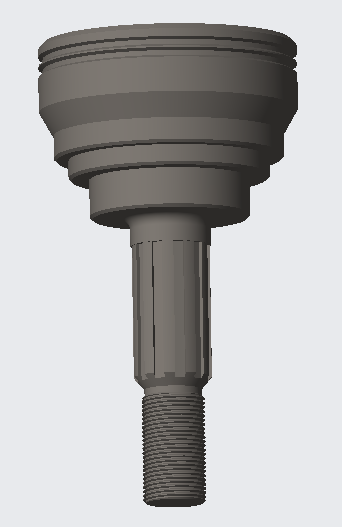
\includegraphics[width=\textwidth]{Immagini/Half-shaft/Half-shaft front.png}
        \caption{Half-shaft end joint upper view}
    \end{minipage}
\end{figure}

\subsection{Design requirements and constraints}
Before detailing the gripper architecture, the geometric and functional constraints dictated by the half-shaft end joint are formally summarized below. These constraints guided every design choice made throughout the development process, including the scrapped attempts discussed in Section~2.

\begin{itemize}
    \item \textbf{Graspable diameter range:} the gripper must accommodate half-shaft sections between $25\text{ mm}$ and $35\text{ mm}$ in diameter, covering approximately $90\%$ of the half-shaft end joints available on the automotive market.
    \item \textbf{No-touch zones:} due to the intricate geometry of the Rzeppa joint (splined input shaft, ball cage, and both threaded sections), most of the component's surface cannot be grasped without risking damage to delicate features. The gripper is therefore restricted to only two contact regions: the intermediate $28\text{ mm}$ non-threaded cylindrical section (claws) and the $23\text{ mm}$ threaded section near the shaft end, which can only be touched axially by the buffer, never radially clamped.
    \item \textbf{Surface protection:} every contact point must be coated with a rubber layer. This is a direct consequence of the no-touch constraint above: since the only accessible surfaces are either toothed or threaded, any rigid metal-on-metal contact would wear down the finish or cause slippage during repeated grasping cycles.
    \item \textbf{Load stability:} because the joint's center of mass is shifted toward the bulkier head, the gripper must counteract the resulting gravity-induced moment to keep the half-shaft horizontal during transport, without relying on structural deformation of the (high-strength metal) component.
    \item \textbf{Compatibility:} the final mechanism must be actuated exclusively through the two linear sliders of the existing \texttt{Jodell} gripper base frame, without introducing additional motors.
\end{itemize}

\subsection{Tray}
The joint is transported in a trail that keeps it horizontal in the same position in which it must be grasped and conserved. Its design facilitates the grasping operation avoiding unnecessary maneuvers.

\subsection{Gripper}
Considering the joint characteristics, the design of the gripper follows two main strategies: 
\begin{itemize}
	\item Ensuring that the part is not damaged during the transport and gripping process: each contact point must have a small rubber layer. In this way, the toothed finishes are not worn out by the repeated grasping process and slips are avoided. Ensuring this will make the robot operate safely.
	\item Compensating the weight forces that, otherwise, would make the joint rotate if picked with the traditional two "fingers": a mechanical buffer is attached on the other side of the contact point of the gripper. This creates a momentum that stabilizes the half-shaft normally affected by gravity forces, not allowing any possible rotations during the transport. In fact, without the buffer part and only using the gripper, the grasp would be unbalanced. 
\end{itemize} 

\subsection{Final design}
The final design consists of an under-actuated mechanical five bar measured to grasp half-shaft end joints with diameters of the grasped section between $25\text{ mm}$ and $35\text{ mm}$, consisting of the $90\%$ of the joints in the automotive market.
Because of this, a simple cylindrical gripper which only performs a rotation about the axis of a single revolute joint (for both sides) is a too simple solution: it would be a cheap and mechanically simple choice, but that would have been the right one only if it were requested to grasp a single type of cylinder, with only one section to care about. To satisfy the task in a robust way, a more complicated quadrilateral-shaped claw was designed by the members of this group.
	\newpage
\section{Design evolution through scrapped designs}

This section has the objective to show the design process of the final component by the various gripper developments, including photos of the claws and occasionally gripper conformations.

\subsection{Static gripper}

In the first stages of development, the main philosophy for the grasping was defined: given the disparity in dimensions in the joint's two main parts, the gripper must act on the smaller side with a motion similar to the gripping of any type of handle. 
To respect this philosophy, a first claw was implemented as a semi-circular crown $5\text{ mm}$ wide and $50\text{ mm}$ long, aiming to completely envelop the small cylinder of the joint. The tampon was also implemented to solve the weight imbalance between the two sides, but the arm was conceived as a solid metal part, rather than sheet metal. The first claw's form is shown below:

\begin{figure}[H]
	\centering
	\begin{minipage}{0.43\textwidth}
		\centering
		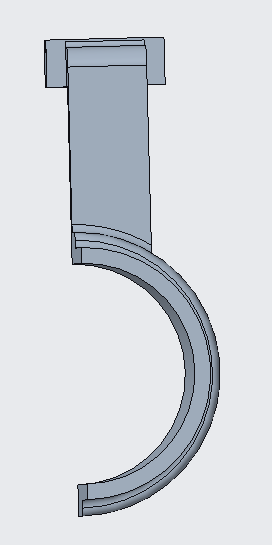
\includegraphics[width=0.5\textwidth]{Immagini/Old models/First claw FW}
		\caption{First claw, front view}
	\end{minipage}
	\hfill
	\begin{minipage}{0.43\textwidth}
		\centering
		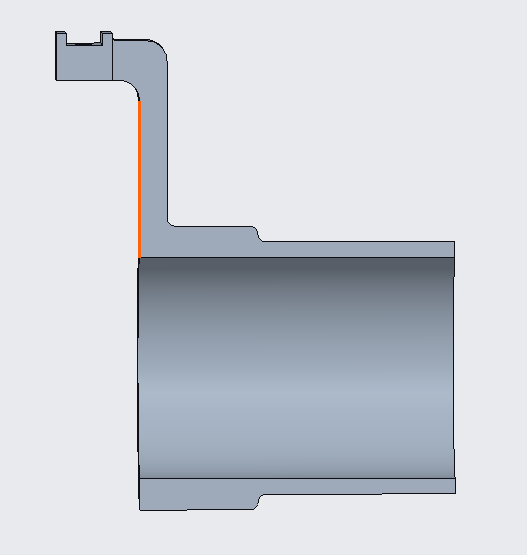
\includegraphics[width=\textwidth]{Immagini/Old models/First claw SW}
		\caption{First claw, side view}
	\end{minipage}
\end{figure}

\begin{figure}[H]
	\centering
	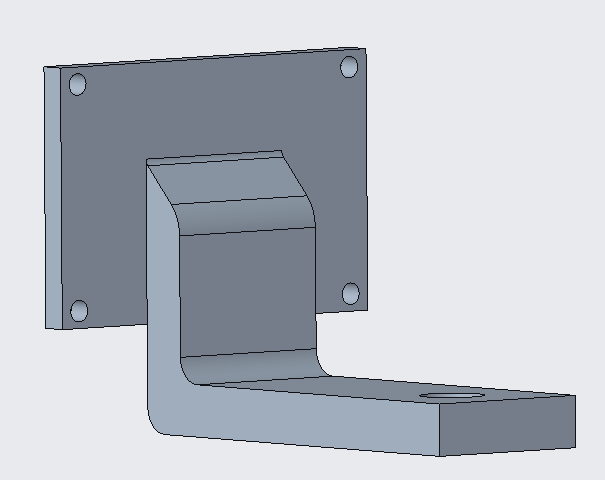
\includegraphics[width=0.5\textwidth]{Immagini/Old models/Braccio}
	\caption{Solid arm}
\end{figure}


Since the joint model used as test subject has a small cylinder circumference of $28\text{ mm}$, this claw was able to grasp it correctly. However, being completely static, the claw was unable to be used in cases where the dimensions would be different than the test radius, which represents an inconvenience in mechanical automated lines.\\
The solid metal arm was also scrapped in favour of a sheet metal structure due to its building complexity in the real world and its negative contribute on weight balancing. 

\subsection{Scrapped arm structures for dynamic claw}

After the failure of the static design, the proposed solution was to use a linkage quadrilateral to let the gripper dynamically reach the component and close itself upon it, following a strict pattern: it is attached on the \texttt{Jodell} component's sliders and moved by those until the proximal link reaches the component; the contact must then force the closing of the quadrilateral around the joint.
This radical change in structure came with tangible challenges and many failed attempts, some of which are reported below: 

\vspace{1cm}
\begin{figure}[H]
	
	\begin{minipage}{0.45\textwidth}
		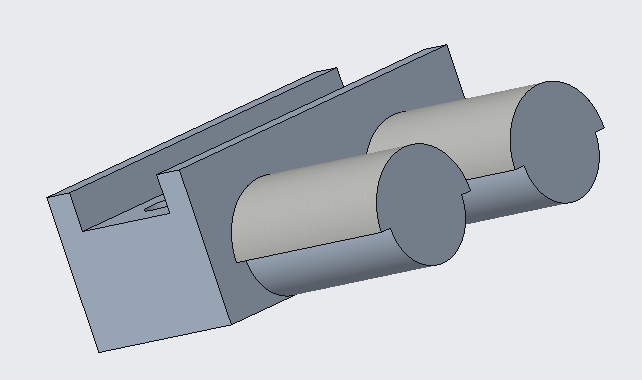
\includegraphics[width=\textwidth]{Immagini/Old models/Base1}
		\caption{Scrapped base for claw}
	\end{minipage}
	\hfill
	\begin{minipage}{0.45\textwidth}
		Here is shown an example of base for a single gripper claw. It uses a $15\times 7\times 6\text{ mm}$ caved block to connect with the \texttt{Jodell}'s sliders and two revolut joints whose exterior is half covered by a $1\text{ mm}$ thick metal coating. This base was scrapped both because the block was too short to actually allow a correct distancing between the two links and because the metal coating on the joints effectively halves the movement freedom for the links. 
	\end{minipage}
	
\end{figure}

\vspace{1cm}

\begin{figure}[H]
	\begin{minipage}{0.35\textwidth}
		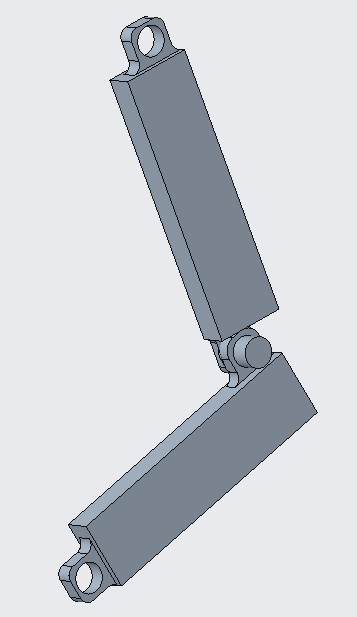
\includegraphics[width=0.9\textwidth]{Immagini/Old models/Arm1}
		\caption{Scrapped model for proximal link}
	\end{minipage}
	\hfill
	\begin{minipage}{0.55\textwidth}
		Here is shown an example of composite proximal link, formed by two solid $3\times 7\times 27\text{ mm}$ links with circle-holed linkages for the revolut joints. The idea was to use the lower link to close on the component when the upper link makes contact with it, but it was scrapped due to several reasons:
		\begin{itemize}
			\item lack of a specific end effector for the gripping;
			\item excessive linkage complexity;
			\item links not thick enough. 
		\end{itemize} 
	\end{minipage}
\end{figure}

\vspace{1cm}
\begin{figure}[H]
	\begin{minipage}{0.37\textwidth}
		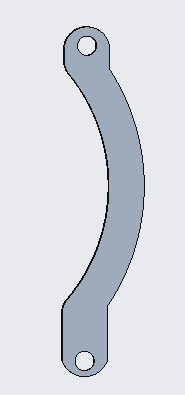
\includegraphics[width=0.6\textwidth]{Immagini/Old models/Arm2}
		\centering
		\caption{Scrapped distal link}
	\end{minipage}
	\hfill
	\begin{minipage}{0.55\textwidth}
		Example of distal link formed with an arch shape between two rounded linkages. Although similar to the final L-shaped distal link, this link was scrapped because of possible collisions with the proximal link when it is moved inwards by the contact with the component. 
	\end{minipage}
\end{figure}

\vspace{1cm}
\begin{figure}[H]
	\begin{minipage}{0.40\textwidth}
		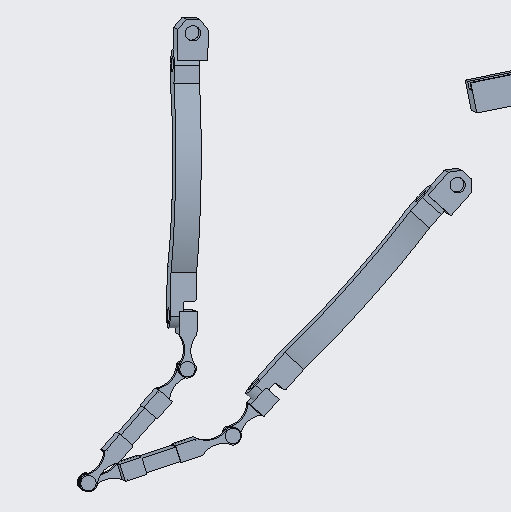
\includegraphics[width=0.8\textwidth]{Immagini/Old models/Gripper1}
		\centering
		\caption{Scrapped claw structure}
		
	\end{minipage}
	\hfill
	\begin{minipage}{0.55\textwidth}
		The claw shown on the left is an example of an embryonal full claw structure formed four straight links and various complex appendages to link them. Despite showing a structure similar to the final one, it was scrapped for problems retained from the component in \texttt{Figure 5}, such as the lack of an end effector and the links being too thin and small. Another issue is caused by the linkages being "jewelry pieces", or pieces too small to be realistically built without loss of resources due to excessive complexity: this pieces were integrated with the links in the final design to form unique pieces that serve all purposes.  
	\end{minipage}
\end{figure}

\vspace{1cm}
\begin{figure}[H]
	
	\begin{minipage}{0.45\textwidth}
		
		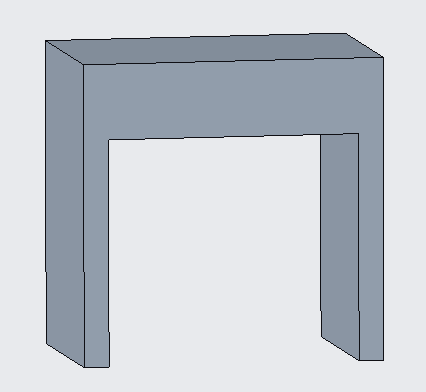
\includegraphics[width=0.8\textwidth]{Immagini/Old models/Anchor}
		\centering
		\caption{Fixed anchor}
	\end{minipage}
	\hfill
	\begin{minipage}{0.50\textwidth}
		Anchor component to be wielded on the \texttt{Jodell} component. It had the objective to slot in the revolut joint for the proximal link. Scrapped in favour of wielding that revolute joint on the base because a fixed anchor limits the movement possibilities of the whole claw.   
	\end{minipage}
\end{figure}

\subsection{Decision matrix: comparison between the scrapped designs and the final solution}
To objectively justify the final choice with respect to the scrapped designs described in this
section, a comparative evaluation matrix is reported below. The criteria considered are
mechanical complexity, grip reliability, adaptability to different component diameters, and ease
of assembly.

\begin{table}[H]
	\centering
	\caption{Evaluation matrix of the scrapped designs versus the final solution}
	\label{tab:decision-matrix}
	\renewcommand{\arraystretch}{1.4}
	\begin{tabular}{|p{3.1cm}|c|c|c|c|p{4.6cm}|}
		\hline
		\rowcolor{black}
		\textcolor{white}{\textbf{Design}} &
		\textcolor{white}{\textbf{Complexity}} &
		\textcolor{white}{\textbf{Reliability}} &
		\textcolor{white}{\textbf{Adaptability}} &
		\textcolor{white}{\textbf{Assembly}} &
		\textcolor{white}{\textbf{Note}} \\
		\hline
		Static gripper (Fig.~5--7) & Low & Low & None & High &
		Fixed grip sized for a single radius; solid metal arm, difficult to manufacture and detrimental to weight balancing. \\
		\hline
		Composite proximal link (Fig.~9) & High & Low & Medium & Low &
		Lack of a dedicated end effector, excessively complex linkage, and links not thick enough. \\
		\hline
		\textbf{Final design} & \textbf{Medium} & \textbf{High} & \textbf{High} & \textbf{Medium} &
		Under-actuated two-claw quadrilateral with return springs and mechanical buffer: good trade-off between adaptability (25--35\,mm) and manufacturing simplicity. \\
		\hline
	\end{tabular}
\end{table}

As highlighted in Table~\ref{tab:decision-matrix}, each of the scrapped designs presented a
critical shortcoming, the lack of adaptability and the excessive linkage
complexity without a dedicated end effector respectively. These hurdles systematically guided the evolution towards
the final solution, capable of balancing adaptability, reliability, and ease of assembly.
	\newpage
\section{Complete mechanism and components description}

In this section it will be explained how the overall final mechanism and each of its components work, including photos from different views for the whole mechanism and the gripper, and a single photo for each component in detail. Dimensions will be indicated as well.

\subsection{Mechanism overview}
From the different views shown in the next page, it can be noticed that the half-shaft end joint is positioned in a perfectly cut slot in the transport tray it is laid on. All the grasping process, whenever the object reaches the destination where it must be lifted, is done by the modified \texttt{Jodell} gripper, which will descend precisely on the shown position to guarantee a solid grip. When the descending phase has ended, it will envelop the non-threaded part of the cylinder, while a buffer positioned on the threaded part (very close to its end) efficiently exerts a force that counters the momentum generated by gravity. The envelop process, carried out by the claws, will only start when the buffer touches the shaft, so that the part will be lifted horizontally. In fact, without it it can be easily assessed that the part would incline in the direction of its centre of mass. Then the gripper will bring the shaft wherever it needs to be in a stabilized way. Every part of the modified gripper that will touch the cylinder is coated with a small rubber layer, as said before. \texttt{Figure 3} was obtained without the tray to give a clearer view of the gripper positioned near to the half-shaft, ready for grabbing. 
\vspace{0.5pt}

\begin{figure}[H]
    \centering
    \begin{minipage}{0.45\textwidth}
        \centering
        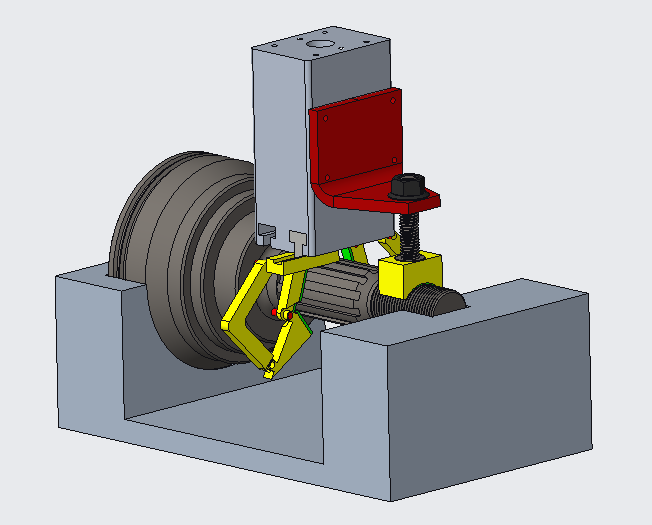
\includegraphics[width=\textwidth]{Immagini/mechanism.png}
        \caption{Mechanism}
    \end{minipage}
    \hfill
    \begin{minipage}{0.45\textwidth}
        \centering
        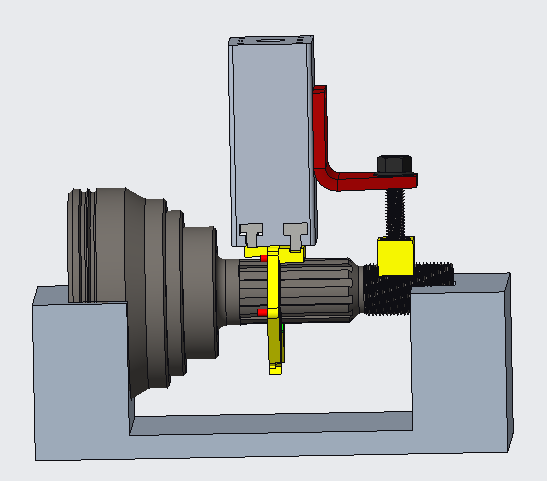
\includegraphics[width=\textwidth]{Immagini/mechanism side.png}
        \caption{Mechanism side view}
    \end{minipage}
\end{figure}

\begin{figure}[H]
    \centering
    \begin{minipage}{0.45\textwidth}
        \centering
        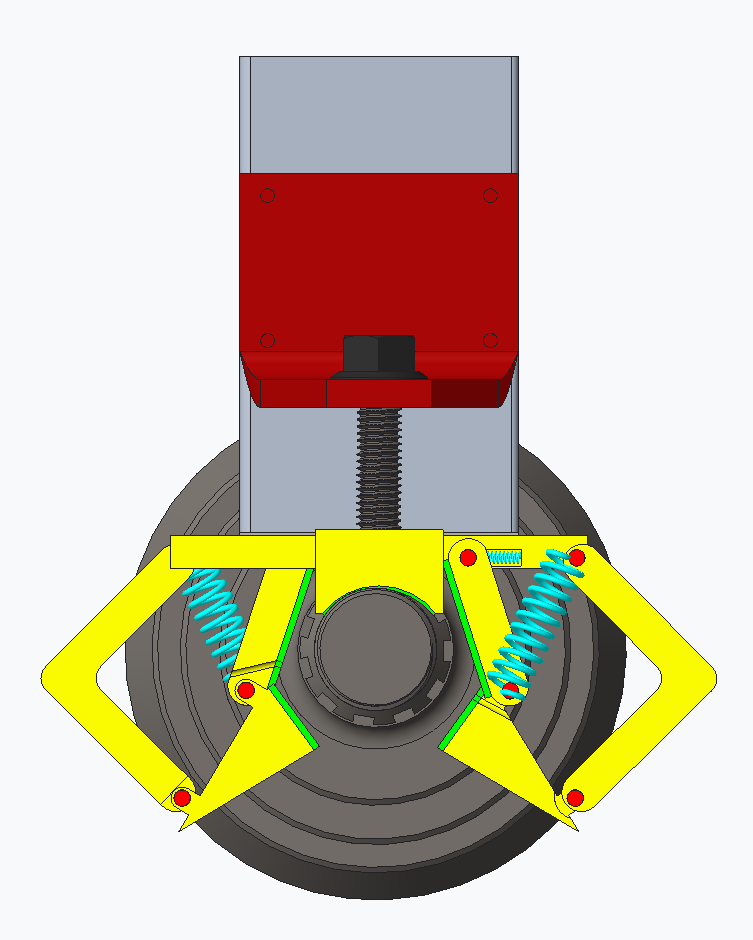
\includegraphics[width=0.7\textwidth]{Immagini/mechanism front.png}
        \caption{Mechanism front view}
    \end{minipage}
    \hfill
    \begin{minipage}{0.45\textwidth}
        \centering
        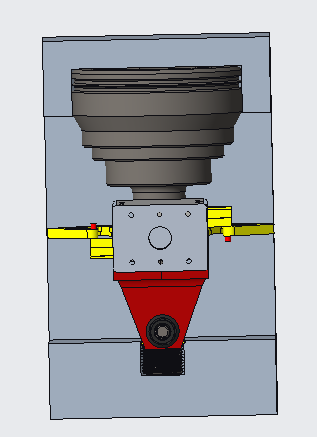
\includegraphics[width=0.7\textwidth]{Immagini/mechanism up.png}
        \caption{Mechanism upper view}
    \end{minipage}
\end{figure}


\subsection{Modified \texttt{Jodell} gripper analysis}
Here, the principal design decision of the \texttt{Jodell} gripper that brought to this definitive design was conditioned by the need to grasp the same object but with different possible section dimensions considering the market availability. The result of a brief research on these dimensions was a range from $25\text{ mm}$ to $35\text{ mm}$, consisting of the $90\%$ of the half-shaft end joints in the automotive market. The internal gum layers are made of high density expanded neoprene and low density expanded polyethylene. As can be seen from \texttt{Figure 8}, the two quadrilateral claws are mounted on two sliders which are positioned in two specific slots. These are put in two grooves created on the base body of the gripper. The functioning process provides that the sliders will bring the proximal links close to the cylinder until they touch it. Then, because of the upper revolute joints and of the way the claws were designed, they will start to envelop the lower part of the cylinder with the triangular pieces. The movement is constrained with springs to resist the gravitational force pushing down the half-shaft end joint during the lift process. 

\begin{figure}[H]
    \centering
    \begin{minipage}{0.49\textwidth}
        \centering
        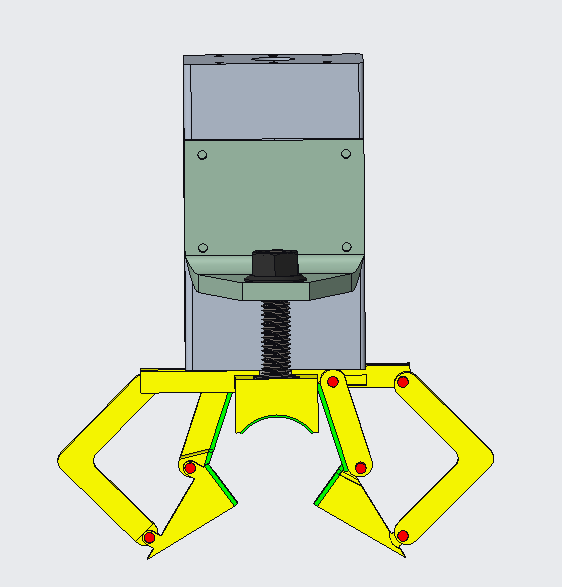
\includegraphics[width=\textwidth]{Immagini/Jodell gripper/jodell fronte.png}
        \caption{\texttt{Jodell} gripper front view}
    \end{minipage}
    \hfill
    \begin{minipage}{0.45\textwidth}
        \centering
        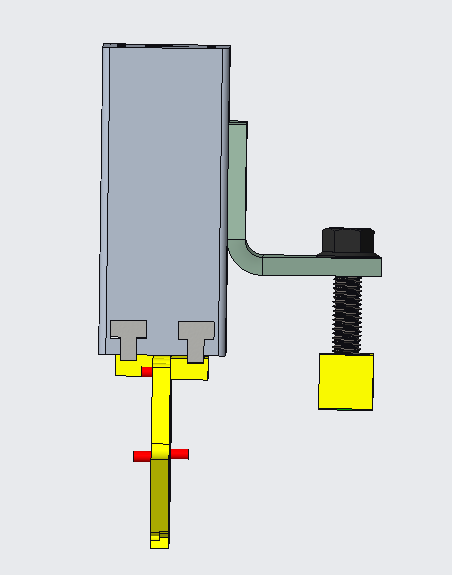
\includegraphics[width=\textwidth]{Immagini/Jodell gripper/jodell side.png}
        \caption{\texttt{Jodell} gripper side view}
    \end{minipage}
\end{figure}

\begin{figure}[H]
    \centering
    \begin{minipage}{0.48\textwidth}
        \centering
        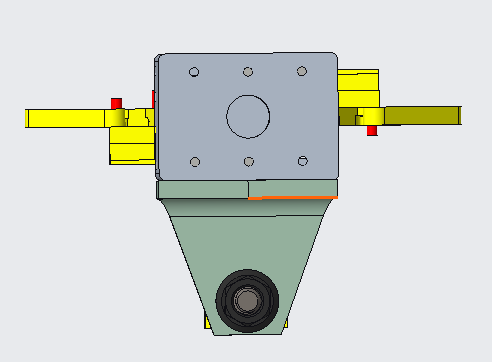
\includegraphics[width=\textwidth]{Immagini/Jodell gripper/jodell alto.png}
        \caption{\texttt{Jodell} gripper upper view}
    \end{minipage}
    \hfill
    \begin{minipage}{0.45\textwidth}
        \centering
        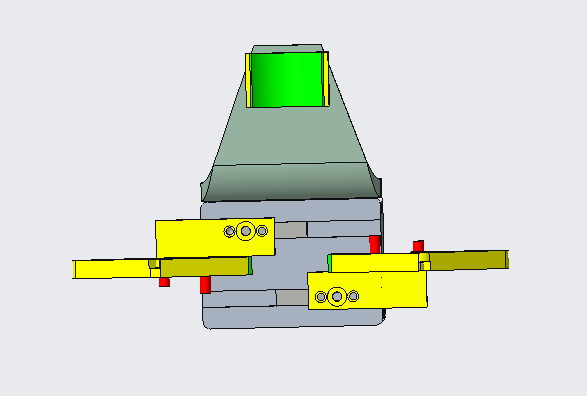
\includegraphics[width=\textwidth]{Immagini/Jodell gripper/jodell sotto.png}
        \caption{\texttt{Jodell} gripper underneath view}
    \end{minipage}
\end{figure}

\subsection{Parts analysis}

\subsubsection{Base of the claw and slider}

Here the main base of the claws can be seen in \texttt{Figure 9}: its upper groove hosts the bottom surface of the slider mounted on the main body of the \texttt{Jodell} gripper (\texttt{Figure 10}). The contact only interests half of both, for functioning purposes, as shown in \texttt{Figure 11}. Then, when the gripper will come in contact with the shaft through the buffer, the \texttt{Jodell} gripper sliders will move on their resting position to the inside until the claws touch the cylinder they are supposed to grasp. The red parts are two revolute joints firstly used to connect the claw to its base, secondly to make it rotate after touching the cylinder with the proximal links of the mechanism. The cubic blue part inside the lateral groove, which houses the shorter revolute joint, is attached to one of the two sprigs per claw. It is useful to compress the spring attached to it when the proximal link has already come in contact with the cylinder. Then, as will be explained later, the slider continues to move along its direction compressing the spring, which allows to keep the proximal link in contact with the cylinder and actuating the rest of the movement of the claws to complete the grasping process.

\begin{figure}[H]
    \centering
    \begin{minipage}{0.30\textwidth}
        \centering
        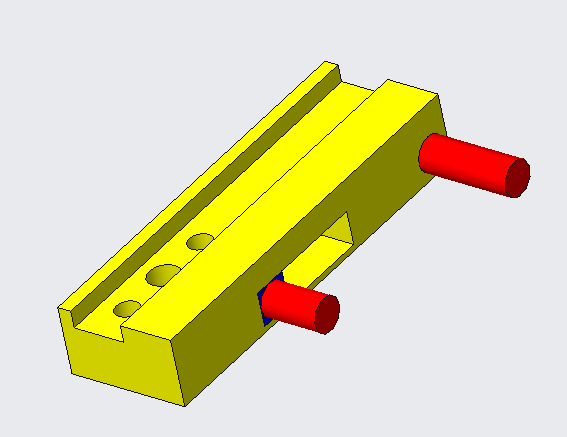
\includegraphics[width=1\textwidth]{Immagini/Jodell gripper/Claw/base claw 2.png}
        \caption{Base of the claw}
    \end{minipage}
    \hfill
    \begin{minipage}{0.30\textwidth}
        \centering
        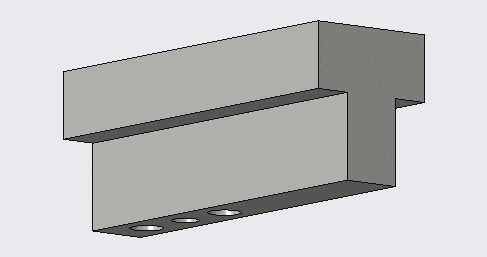
\includegraphics[width=1\textwidth]{Immagini/Jodell gripper/Claw/gripperconnector.png}
        \caption{Slider}
    \end{minipage}
    \hfill
    \centering
    \begin{minipage}{0.30\textwidth}
    	\centering
    	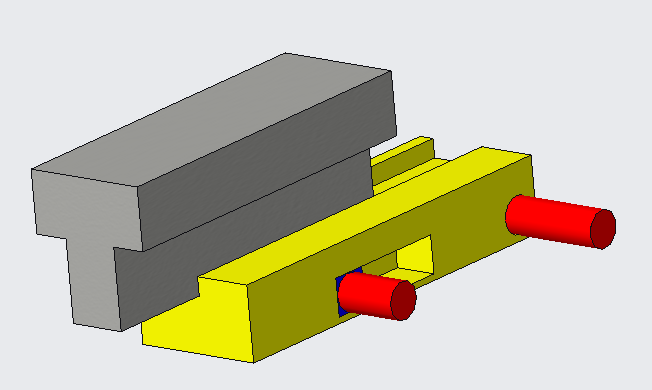
\includegraphics[width=1\textwidth]{Immagini/Jodell gripper/Claw/slider + base.png}
    	\caption{Claw base mounted on the slider}
    \end{minipage}
    
\end{figure}

The sliding base has a dimension of $35\text{ mm}$ when at rest, defining a trapezoidal mechanism, while it has a dimension of $25\text{ mm}$ at maximum compression (when the cylinder is touched only with a sliding movement). The useful stroke of the slider corresponds to $10$--$12\text{ mm}$.

\vspace{0.5cm}
\subsubsection{Proximal link, distal link and triangular hugger}

\begin{figure}[H]
    \begin{minipage}{0.45\textwidth}
        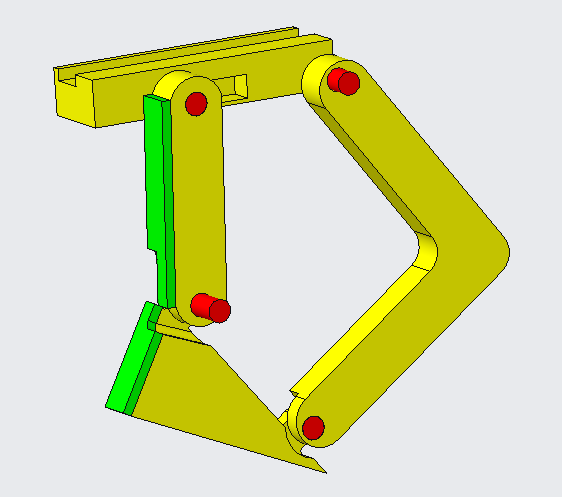
\includegraphics[width=\textwidth]{Immagini/Jodell gripper/Claw/claw3.png}
        \caption{Claw mechanism}
    \end{minipage}
    \hfill
    \begin{minipage}{0.45\textwidth}
    Here is shown the complete mechanism of the claw, whose task is to basically hug the shaft cylindrical part to securely lift it (cooperating with the buffer). Every part that composes it can be clearly seen: the base of the claw housing the slider of the \texttt{Jodell}, the shorter proximal link (the first to touch the cylinder), the longer L-shaped distal link and the triangular hugger, which is fundamental to correctly perform the grasp.
    \end{minipage}
\end{figure}

\begin{figure}[H]
    \begin{minipage}{0.35\textwidth}
        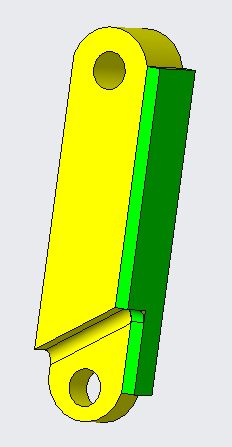
\includegraphics[width=0.7\textwidth]{Immagini/Jodell gripper/Claw/prossimale.png}
        \centering
        \caption{Proximal link}
    \end{minipage}
    \hfill
    \begin{minipage}{0.55\textwidth}
    The shorter, proximal link (\texttt{Figure 13}) is the first to come in contact with the shaft cylinder. The touch happens in two phases: the first only after a sliding movement of the slider mounted on the main body of the \texttt{Jodell}, until the proximal link touches the cylindrical part of the shaft. The second phase begins when, having the link already in contact, it is maintained like that by the spring in the base of the claw.
    The contact surface is covered with a thin layer of elastic rubber-like material (as said in the description of the \texttt{Jodell} modified manipulator at page $2$). The direct distance between the holes (that will host the revolute joints) measures $45\text{ mm}$.
    \end{minipage}
\end{figure}

\begin{figure}[H]
    \begin{minipage}{0.4\textwidth}
        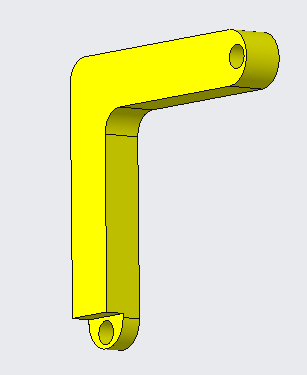
\includegraphics[width=0.8\textwidth]{Immagini/Jodell gripper/Claw/distalee.png}
        \centering
        \caption{Distal link}
    \end{minipage}
    \hfill
    \begin{minipage}{0.55\textwidth}
    As the claw keeps sliding, the rest of the mechanism performs a rotation movement to envelop the bottom surface of the cylinder itself. The main protagonists are the distal link (\texttt{Figure 14}) and the triangular hugger (\texttt{Figure 15}). Here, the distal link allows the hugger to perform the required rotation movement together with the movement of each other part. It as a L-shaped (or elbow-shaped) structure where the tip of it needs to stick out of $20\text{ mm}$ from the line connecting the centers of the two holes, to create the cradle that accommodates a diameter dimension of $35\text{ mm}$ without bumps. The direct distance between the holes (that will host the revolute joints) measures $45\text{ mm}$.
    \end{minipage}
\end{figure}

\begin{figure}[H]
    \begin{minipage}{0.40\textwidth}
        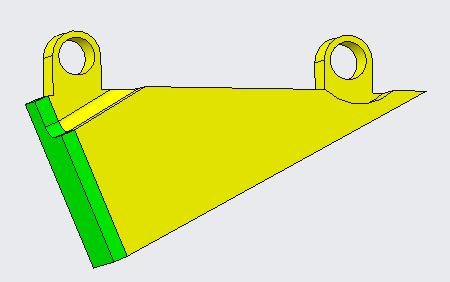
\includegraphics[width=\textwidth]{Immagini/Jodell gripper/Claw/triangolo.png}
        \centering
        \caption{Triangular hugger}
    \end{minipage}
    \hfill
    \begin{minipage}{0.55\textwidth}
    The triangular hugger here is the last component of the claw which makes the mechanism a closed one, the shorter side is the one which comes in contact with the surface of the cylinder together with the proximal link, so it is coated with the same rubber layer. The distance between the holes measures $25\text{ mm}$. It can be seen from the image that two grooves were performed on the surface near the holes. That is made to avoid collisions with the two links above it during the rotation.
    \end{minipage}
\end{figure}

\subsubsection{Springs utilization}
\label{sec:springs}

\begin{figure}[H]
    \centering
    \begin{minipage}{0.45\textwidth}
        \centering
        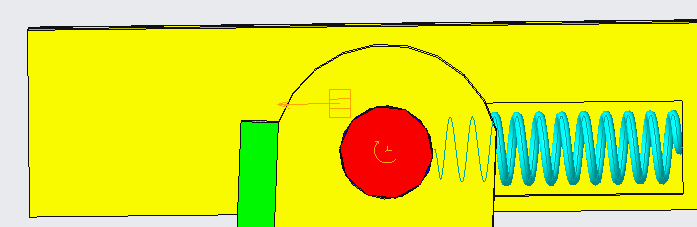
\includegraphics[width=\textwidth]{Immagini/Jodell gripper/Claw/molle1.png}
        \caption{First spring in the base of the claw}
    \end{minipage}
    \hfill
    \begin{minipage}{0.50\textwidth}
        \centering
        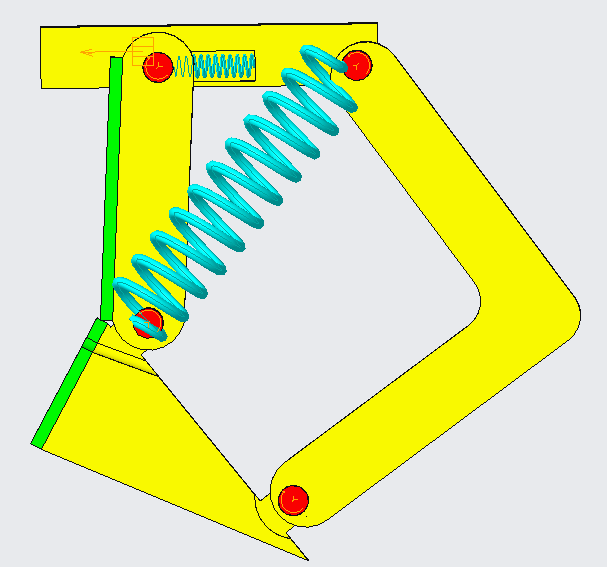
\includegraphics[width=\textwidth]{Immagini/Jodell gripper/Claw/molla2.png}
        \caption{Second spring between the hugger and the distal link}
    \end{minipage}
\end{figure}

All the springs, shown only via the \texttt{Creo Mechanism} window, serve two purposes:
\begin{itemize}
	\item \texttt{\textbf{When not in contact:}} to keep the claws in a constant stable position, to ensure the correct initialization of the robot actions. This position is kept stable during the approaching phase of the claw to the cylinder, in order to generate the first contact between it and the proximal link. 
	\item \texttt{\textbf{When in contact:}} to grant the adaptability of the mechanism and the dynamic of the movement. During this phase, the action of the springs allows the links to rotate in such way to correctly envelop the cylinder, keeping the grip stabilized. While in the first phase only a translational movement interested the links of the claw, during the second phase rotational movements are the main ones.

\end{itemize}

\vspace{1cm}
\subsubsection{Mechanical buffer}

The second part of the modified gripper consists of the stabilization system which is formed by the mechanical buffer (\texttt{Figure 18}). It helps to stabilize the positioning of the shaft when lifted by maintaining it in a horizontal position during all the movement. More precisely, this happens by only touching the threaded part of the cylindrical portion of the half-shaft with its rubber end, which will generate a resisting force that will counter the momentum generated by the gravity force. In fact, the physical constitution of the half-shaft clearly shows that the centre of mass is placed near the part with the biggest section. This surely makes the piece tilt when trying to lift it only with the claw part of the gripper, because of the gravity force. So it is needed a stabilization system like it was designed.
Mechanically, it is composed by a sheet metal mounted on the side of the \texttt{Jodell} main body (\texttt{Figure 22}), a M8 nut with flange and a thread pitch of $1{,}25$ (\texttt{Figure 20}), a screw of the type DIN 912 M8X30F A2 (same thread pitch of the nut) (\texttt{Figure 19}) and a rubber extremity (\texttt{Figure 21}). The sheet metal represents the fixed support on which the rest of the buffer is built. In fact, a hole of diameter $7{,}5\text{ mm}$ was created at the extremity of the horizontal part of the sheet metal. The screw has a diameter of $8\text{ mm}$ so the slightly restricted section of the hole allows a solid fit. The screwing distance can be regulated basing on the correct positioning of the gripping part, considering that the maximum length of the screwable part is of $30\text{ mm}$ measured from the screw head. To better stabilize the screw, a nut with a flange ($8\text{ mm}$ in diameter) is put on top of the hole laying on the sheet metal in that position. Then, the rubber swab has a hole carved in to house the head of the screw. The diameter of the head is $12{,}4\text{ mm}$. 


\begin{figure}[H]
	\vspace{2cm}
    \centering
    \begin{minipage}{0.30\textwidth}
        \centering
        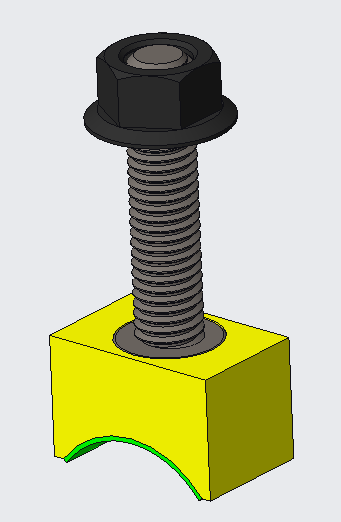
\includegraphics[width=\textwidth]{Immagini/tampone/tampone full.png}
        \caption{Mechanical buffer}
    \end{minipage}
    \hspace{3cm}
    \begin{minipage}{0.25\textwidth}
        \centering
        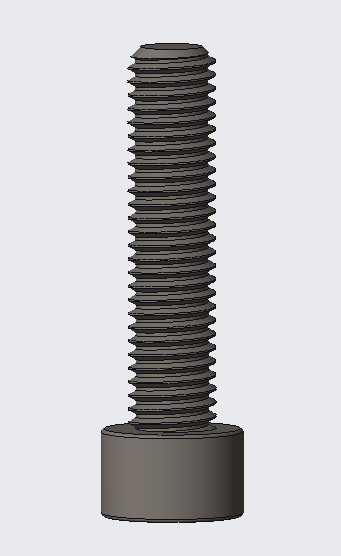
\includegraphics[width=\textwidth]{Immagini/tampone/vite.png}
        \caption{DIN 912 M8X30F A2 screw}
    \end{minipage}
\end{figure}

\begin{figure}[H]
    \centering
    \begin{minipage}{0.30\textwidth}
        \centering
        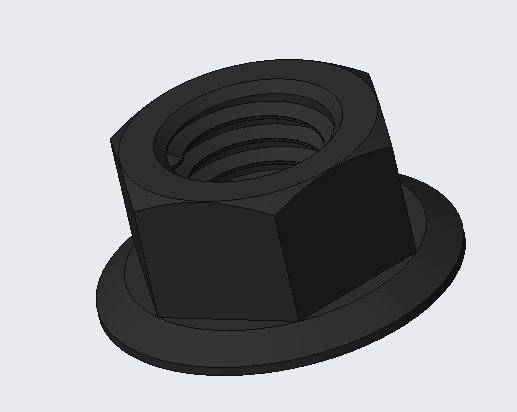
\includegraphics[width=\textwidth]{Immagini/tampone/dado.png}
        \caption{M8x1,25 nut with flange}
    \end{minipage}
    \hspace{2cm}
    \begin{minipage}{0.30\textwidth}
        \centering
        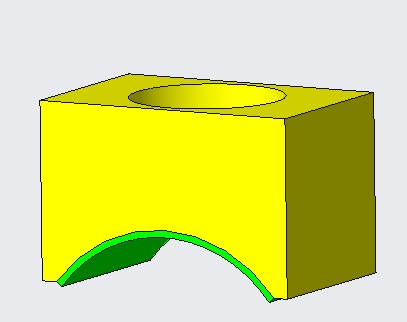
\includegraphics[width=\textwidth]{Immagini/tampone/tampone.png}
        \caption{Rubber swab}
    \end{minipage}
\end{figure}

\begin{figure}[H]
    \centering
    \begin{minipage}{0.35\textwidth}
        \centering
        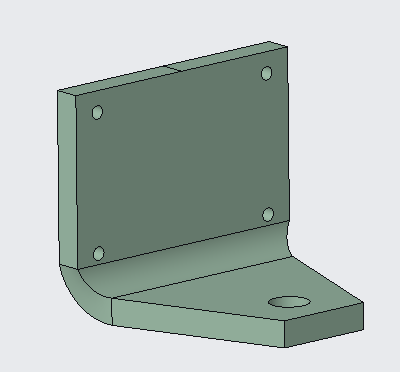
\includegraphics[width=\textwidth]{Immagini/tampone/braccio.png}
        \caption{Sheet metal}
    \end{minipage}
    \hspace{2cm}
    \begin{minipage}{0.35\textwidth}
        \centering
        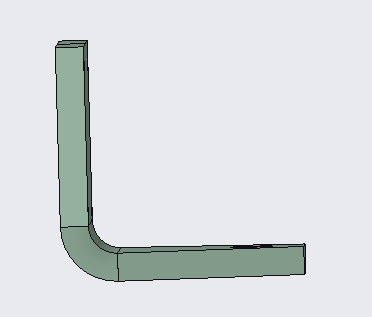
\includegraphics[width=\textwidth]{Immagini/tampone/braccio side.png}
        \caption{Sheet metal side view}
    \end{minipage}
\end{figure}

\vspace{4cm}
\subsubsection{Kinematic closing sequence}
The claw mechanism described above can be summarized as a serial kinematic chain composed of one prismatic pair and three revolute pairs (P--R--R--R): the prismatic pair corresponds to the \texttt{Jodell} slider, while the three revolute pairs connect, in sequence, the claw base to the proximal link, the proximal link to the distal link, and the distal link to the triangular hugger. The closing action unfolds in the following steps:

\begin{enumerate}
    \item \textbf{Linear actuation (P):} the \texttt{Jodell} sliders translate rigidly toward the half-shaft, carrying the claw bases and the buffer support along a purely linear trajectory.
    \item \textbf{Contact and stabilization:} the buffer's rubber end is the first element to reach the shaft, touching the threaded section and generating the counter-moment needed to keep the half-shaft horizontal before any radial grasping force is applied.
    \item \textbf{Passive envelopment (R--R--R):} once the proximal link makes contact with the cylindrical section, the reaction force compresses the base spring (Section~\ref{sec:springs}), which in turn actuates the rotation of the distal link and triangular hugger about their revolute joints, wrapping the claw around the shaft until the grasp is complete.
\end{enumerate}

This sequence highlights that only the first phase is actively driven by the \texttt{Jodell} motor, while the remaining degrees of freedom are closed passively through the spring-loaded linkage, consistently with the under-actuated nature of the mechanism.

\subsubsection{Tray}
The tray is where the half-shaft is placed on. It contains two semi-circular carved parts which have the same sections of the respective ends of the object it must contain. Respectively, the sections measure $90\text{ mm}$ for the head of the shaft slot diameter and $23\text{ mm}$ for the threaded end slot diameter. The lateral vertical sides of the tray extremities are not carved because they must not allow horizontal movements of the shaft during the transport. All of this can be seen in the subsequent images. 

\begin{figure}[H]
    \centering
    \begin{minipage}{0.65\textwidth}
        \centering
        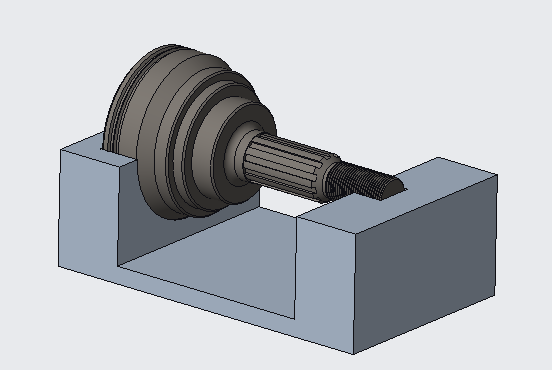
\includegraphics[width=\textwidth]{Immagini/vassoio/vassoio con pezzo.png}
        \caption{Tray containing the half-shaft}
    \end{minipage}
\end{figure}

\begin{figure}[H]
    \centering
    \begin{minipage}{0.65\textwidth}
        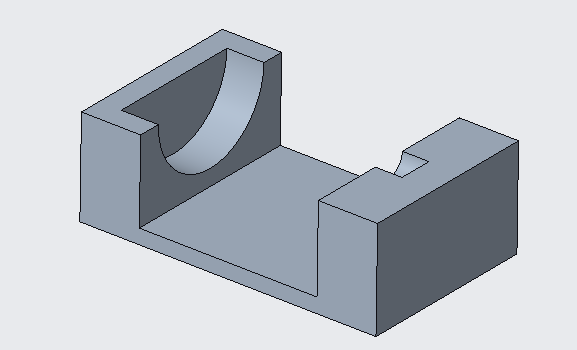
\includegraphics[width=\textwidth]{Immagini/vassoio/vassoio.png}
        \caption{Empty tray}
    \end{minipage}
\end{figure}

\subsection{Parts assembly}

This subsection shows how the components explained in this chapter are assembled to form the final design. This is done by using Creo Parametric's View functionality, more specifically using explode views that allow the components to be temporarily separated without harming the real assembly. For the sake of simplicity and to avoid excessive cluttering, the explode view is shown below both for the singular claw and for the jodell component with the whole claws.

\begin{figure}[H]
	\centering
	\begin{minipage}{0.35\textwidth}
		\centering
		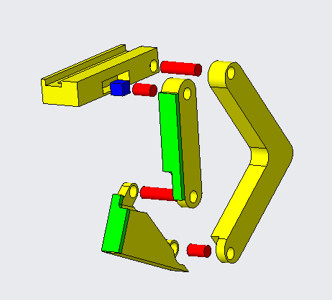
\includegraphics[width=\textwidth]{Immagini/claw_anchorless_espl}
		\caption{Claw exploded view}
	\end{minipage}
	\hspace{2cm}
	\begin{minipage}{0.35\textwidth}
		\centering
		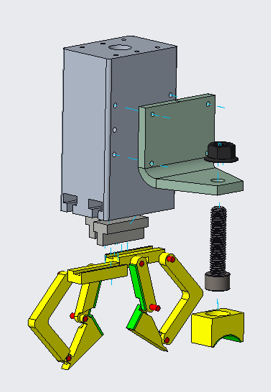
\includegraphics[width=\textwidth]{Immagini/jodell_espl}
		\caption{Jodell assembly exploded view}
	\end{minipage}
\end{figure}

\subsection{Requirement verification}
This section verifies how the final design presented above satisfies the requirements and constraints formally introduced in Section~1.2.

\begin{table}[H]
\centering
\caption{Requirement verification table}
\label{tab:requirement-verification}
\renewcommand{\arraystretch}{1.4}
\begin{tabular}{|p{2.7cm}|p{4.6cm}|p{6.2cm}|}
\hline
\rowcolor{black}
\textcolor{white}{\textbf{Requirement}} &
\textcolor{white}{\textbf{Description}} &
\textcolor{white}{\textbf{How it is satisfied}} \\
\hline
Diameter range & Grasp sections between $25$--$35\text{ mm}$ & The under-actuated quadrilateral claw, combined with the $10$--$12\text{ mm}$ slider stroke, closes on any diameter within this range without manual reconfiguration. \\
\hline
No-touch zones & Avoid splines, ball cage and both threaded sections & The claws contact only the $28\text{ mm}$ non-threaded cylindrical section, while the buffer contacts the $23\text{ mm}$ threaded section exclusively along its axis, never radially. \\
\hline
Surface protection & Prevent wear and slipping on delicate finishes & Every contact point (claws, hugger, buffer tip) is coated with a rubber layer that absorbs clamping force and prevents metal-on-metal contact. \\
\hline
Load stability & Counteract the gravity-induced moment caused by the off-centered mass & The mechanical buffer engages the threaded section before the claws close, generating a counter-moment that keeps the half-shaft horizontal throughout the lift. \\
\hline
Compatibility & Operate using only the \texttt{Jodell} linear sliders & The whole claw kinematics (P--R--R--R chain, Section~3.3.4) is driven by the two existing sliders; no additional actuator was introduced. \\
\hline
\end{tabular}
\end{table}

    \newpage
\section{Conclusions}
To conclude, the proposed gripper represents a good compromise between functionality, adaptability and manufacturing simplicity. The final solution satisfies the main requirements defined at the beginning of the project, allowing the component to be grasped from the safe lower cylindrical surface while avoiding the restricted areas.

The two-claw under-actuated quadrilateral architecture, together with the replaceable rubber attachments and the simplified mechanical structure, supports a stable pick-up, easy maintenance and a feasible assembly process. For these reasons, the design can be considered suitable for the required task.

Finally, the final CAD test confirms that the gripper can close correctly, as seen in the test below, conducted with the component with the largest diameter. The claws remain aligned with the safe contact areas and avoid interference with the flanges, validating the design approach used.

\begin{figure}[H]
	\centering
	\begin{minipage}{0.45\textwidth}
		\centering
		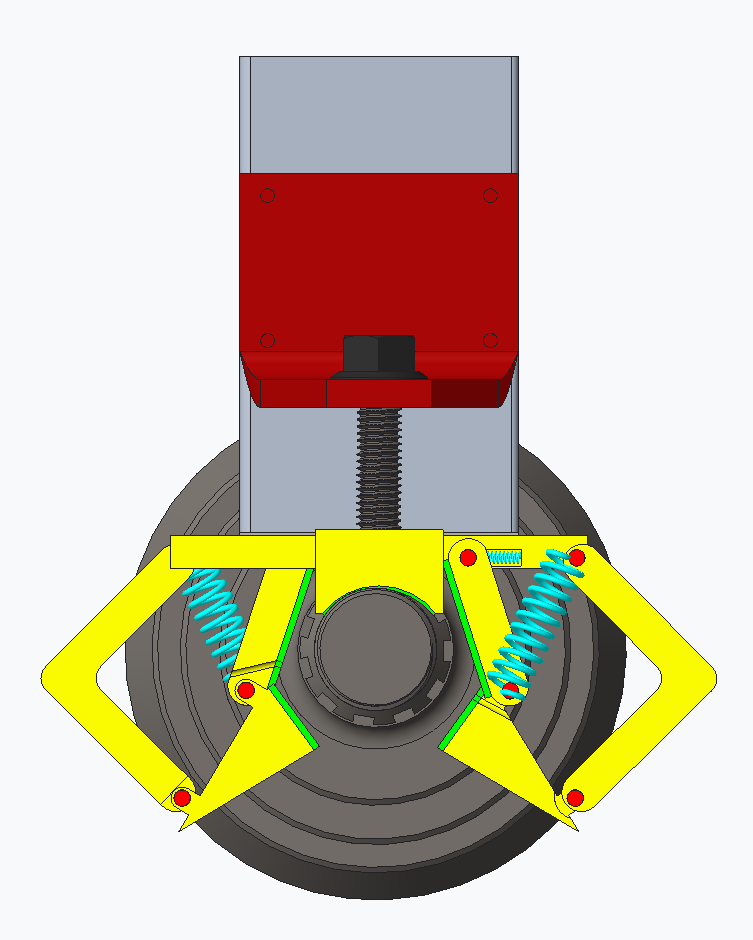
\includegraphics[width=\textwidth]{Immagini/mechanism front.png}
		\caption*{Test start:\\ the gripper has enough tolerance prior to motion}
	\end{minipage}
	\hfill
	\begin{minipage}{0.45\textwidth}
		\centering
		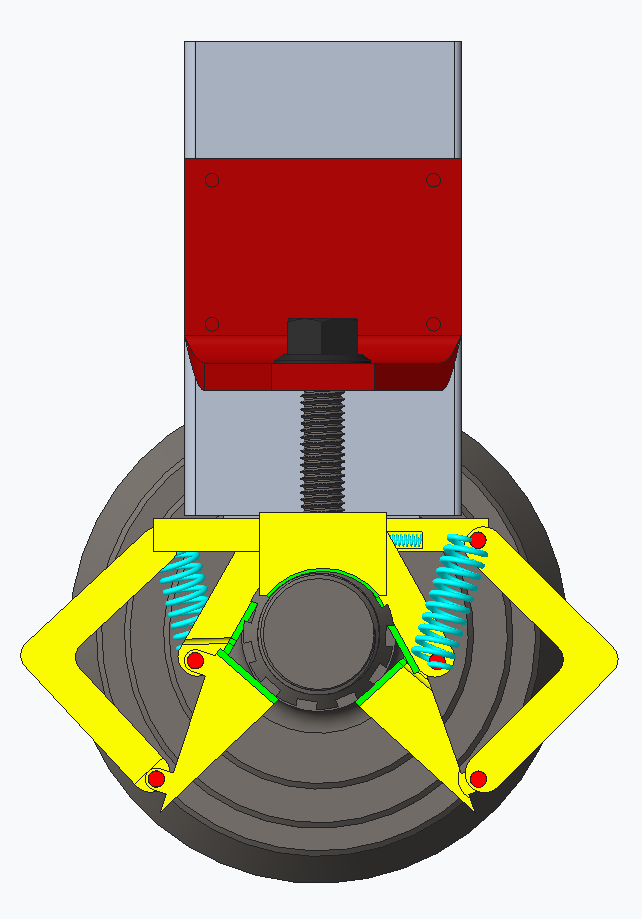
\includegraphics[width=\textwidth]{Immagini/tennis.png}
		\caption*{Test end:\\ the rubber ensures enough pressure on the component to guarantee better pick up}
	\end{minipage}
\end{figure}

\subsection*{Possible future adjustments for Manufacturing}
The following are possible future design improvements to reduce costs and increase ease of manufacturing:
\begin{itemize}
	\item Modify and make the links in sheet metal rather than steel as in the current version.
	\item Perform cuts to further reduce material at various points of the design, such as in the lateral supports.
	\item Add laser cuts also in the bases of the two rotating claws to facilitate the assembly of the part.
	\item Add a metal notch inside the rubber of the claw tips to improve the stability and firmness of the grip.
\end{itemize}
    
	\pagebreak
	
\end{document}
